%% LaTeX template for diploma thesis at the 
%% department of civil and environmental engineering of TU Wien
%% Following files have to be in the same directory:
%% TUWBUIDADISS.sty and tuw-bui-logo-2022.pdf
%% 
%% created by Christian Schranz and Sebastian Pech
%% CEE Computer Lab & Digital Building Process
%% date: 2022-10-01
%% tested for pdflatex
%%

%Hierarchie der Überschriften
%\section{}
%\subsection{}
%\subsubsection{}
%\paragraph{}
%\minisec{} Kann man für kleine Überschriften ohne Nummerierung verwenden

\pdfminorversion=7

%% ========== TITLE INFORMATION ==========
\newcommand{\thesistype}{DA} 
\newcommand{\thesislanguage}{de-AT}
\newcommand{\thesistitle}{Entwicklung und Dokumentation einer kostengünstigen Anzeigelösung für Lüftungsanlagen auf Basis des "Modbus"-Protokolls}
\newcommand{\fenkart}{Lukas Fenkart}
\newcommand{\mangeng}{Luca jerome Mangeng}
\newcommand{\pezze}{Damiano Pezzè}
\newcommand{\schneider}{Martin Schneider}


\documentclass[12pt,twoside=false, a4paper]{scrreprt}


\usepackage[utf8]{inputenc}
\usepackage{TUWBUIDADISS}
%% this style alreadz includes some useful packages:
%% fontenc[T1], lmodern, microtype, babel[englisch,ngerman], graphicx, 
%% geometry with all margins or areaset (choose what you like)
%% mathtools, amssymb, xfrac, siunitx, booktabs,
%% url, xcolor[table], textcomp, marvosym, pifonts, pdfpages, ragged2e, 
%% tabularx, longtable, threeparttable, csquotes, eurosym, enumitem, 
%% multirow, setspace, listings, scrlayer-scrpage with header/footline
%% pdfx (including hyperref)

\raggedbottom 
%% prevents the expansion of the text till the end of the page (if you like)
%\setcapindent{0em} %% influences captions layout
%%
%% ========== Key Words ==========
%%
%% Geben Sie beim Befehl \Keywords einige Key Words ein und 
%% trennen Sie diese mit dem Befehl \sep%%
\begin{filecontents}[overwrite]{\jobname.xmpdata}
\Language{\thesislanguage}
\Title{\thesistitle}
\Keywords{diploma thesis\sep template\sep LaTeX}
\end{filecontents}

%% use biblatex and biber for bibliography
%% customize options as you like
%% style=numeric-comp ... [1]
%% style=authoryear ... Mang 1998 / use \textcite{} ... Mang (1998)
%%
\usepackage[style=numeric-comp,backend=biber,maxcitenames=2]{biblatex}
\ExecuteBibliographyOptions{%
  giveninits=true,maxbibnames=99}%
\DefineBibliographyStrings{ngerman}{andothers={et\;al\adddot},
urlseen = {Zugriff am}}
\addbibresource{Literatur.bib}


%% ===== additional packages to the ones already loaded ==============
\usepackage{acro}
%\ac{Kuerzel} wird der Befehl \ac{Kuerzel} das erste Mal verwendet, erhält man die Langform des Ausdrucks und zusätzlich die geklammerte Kurzform. Wird der Befehl danach wieder mit dem gleichen Kürzel, erhält man die Kurzform dann aber ohne Klammern.
%\acl{Kuerzel} schreibt die Langform des Ausdrucks.
%\acs{Kuerzel} schreibt die Kurzform.
%\aclp{Kuerzel} schreibt die Langform des Plurals des Ausdrucks.
%\acsp{Kuerzel}schreibt die Kurzform des Plurals. 
%\acf{Kuerzel} verhält sich wie \ac{Kuerzel} Befehl, wenn er das erste Mal aufgerufen wurde. Unabhängig davon, wie oft das Kürzel bereits aufgerufen wurde, wird bei der Verwendung von \acf{Kuerzel} die ausgeschriebene Langform des Ausdrucks und die geklammerte Abkürzung gesetzt.

\DeclareAcronym{obv}{
short = {\"obv},
long  = {Österreichische Bautechnikvereinigung},
}

\DeclareAcronym{dt}{
short = {dt.},
long  = {deutsch},
}

\DeclareAcronym{engl}{
	short = {engl.},
	long  = {englisch},
}

\DeclareAcronym{python}{
	short = {Python},
	long  = {},
}

\DeclareAcronym{abbv}{
short = {ABBV},
long  = {Ablösungsbeträge-Berechnungsverordnung},
short-plural = {s},
long-plural = {en},
}

\DeclareAcronym{lzk}{
short = {LZK},
long  = {Lebenszykluskosten},
extra = {[\officialeuro{}]},
}

\DeclareAcronym{rlt}{
	short = RLT,
	long  = raumlufttechnische,
	short-plural = s,
	long-plural = n,
}

\DeclareAcronym{rltanlage}{
	short = RLT Anlage,
	long  = raumlufttechnische Anlage,
	short-plural = n,
	long-plural-form = raumlufttechnische Anlagen,
}

\DeclareAcronym{rltanlagen}{
	short = RLT Anlagen,
	long  = raumlufttechnische Anlagen,
}

\DeclareAcronym{gui}{
	short = GUI,
	long  = Grafische Benutzeroberfläche,
	short-plural = s,
	long-plural = n,
}

\DeclareAcronym{htl}{
	short = HTL,
	long  = Höhere Technische Bundeslehr- und Versuchsanstalt,
}

\DeclareAcronym{json}{
	short = \gls{gls_json},
	long  = JavaScript Object Notation,
}

\DeclareAcronym{csv}{
	short = \gls{gls_csv},
	long  = Comma-Separated Values,
}

\DeclareAcronym{rfc}{
	short = RFC,
	long  = Request for Comments,
}

\DeclareAcronym{mime}{
	short = MIME-Type,
	long  = Internet Media Type,
}

\DeclareAcronym{crlf}{
	short = CRLF,
	long  = Carriage Return Line feed,
}

\DeclareAcronym{pdu}{
	short = PDU,
	long = Protocol Data Unit,
}

\DeclareAcronym{adu}{
	short = ADU,
	long = Application Data Unit,
}

\DeclareAcronym{tcp}{
	short = TCP,
	long = Transmission Control Protocol,
}

\DeclareAcronym{rtu}{
	short = RTU,
	long = Remote Terminal Unit, 
}

\DeclareAcronym{ascii}{
short = ASCII,
long = American Standard Code for Information Interchange, 
}

\DeclareAcronym{io}{
	short = I/O System,
	long = Input/Output System, 
}

\DeclareAcronym{rltanzeige}{
	short = RLT Anzeige,
	long = Raumlufttechnische Anzeige,
}

\DeclareAcronym{crc}{
short = CRC,
long = Cyclical Redundancy Checking, 
}

\DeclareAcronym{lrc}{
short = LRC,
long = Longitudinal Redundancy Checking, 
}

\DeclareAcronym{xml}{
	short = XML,
	long = Extensible Markup Language,
}




%% Einstellungen für Zeilenumbrüche von Weblinks im url-Paket
\setcounter{biburllcpenalty}{9000}% Kleinbuchstaben
\setcounter{biburlucpenalty}{9000}% Großbuchstaben
%% Quelle: https://texwelt.de/fragen/7008/zeilenumbruche-in-bibliografielinks

%% ===== additional settings =============
\setcounter{secnumdepth}{3}
\sisetup{output-decimal-marker = {,},
range-phrase = --,
group-separator = {~},
per-mode = symbol, 
list-final-separator={ und }}

\graphicspath{{Bilder/}}

%% examples for useful shortcuts in German
\newcommand{\zB}{\mbox{z.\,B.}\xspace}
\newcommand{\Name}[1]{\textsc{#1}}

\newcommand{\vKTxv}{\mathbf{v}_1^T\tilde{\mathbf{K}}_{T},_{\xi}\mathbf{v}_1}
\newcommand{\vKTxxv}{\mathbf{v}_1^T\tilde{\mathbf{K}}_{T},_{\xi\xi}\mathbf{v}_1}

% activate for double space between the lines (correction mode) 
%\doublespacing

\begin{document}       %% start of the document
\maketitle             %% places the title with above information

\cleardoublepage
\selectlanguage{ngerman}  %% for german abstract
\chapter*{Kurzfassung}
      %% german abstract

\cleardoublepage
\selectlanguage{english}    %% for english abstract
\include{00-abstract}         %% english abstract

%\cleardoublepage
\selectlanguage{ngerman} 
\pagestyle{scrheadings} 

\tableofcontents

\chapter{Beispiele}

In diesen Dateien finden Sie die Beispiele aus den youtube-Videos:

\url{https://www.youtube.com/playlist?list=PLwlC-XZXtzhg4fQiZQAsXIMSRW-iZtnTQ}

\section{section bsp}
\begin{figure}
	\centering
	
\includegraphics[width=0.4\linewidth]{Bilder/HTL_Dornbirn_Logo}
	\caption{HTL Dornbirn Logo (Quelle: \url{https://www.htldornbirn.at/})}
	\label{fig:htldornbirnlogo}
\end{figure}


\section{Beispiele aus dem Video zur Bachelorarbeit}
\setAuthor{\pezze}
\minisec{Tipps: Schreiben einer wissenschaftlichen Arbeit mit \LaTeX{}}
%
Generell stellt sich für uns das Problem, nun mit \LaTeX{} einfach und rasch eine wissenschaftliche Arbeit zu schreiben.
Den Inhalt nimmt uns \LaTeX{} leider nicht ab, dafür sind wir selbst verantwortlich.
Jedoch können wir uns bei \LaTeX{} auf einige Vorteile verlassen, die wir hier näher betrachten möchten.
Vorweg sei die konsistente Formatierung genannt.

Bevor wir diese Vorteile behandeln, beschäftigen wir uns mit generellen Anforderungen an wissenschaftliche Arbeiten.
Die Erstellung der Gliederung und des Aufbaus einer wissenschaftlichen Arbeit sind meist der erste Schritt für jede Autorin bzw. jeden Autor.
Danach beschäftigt uns der Inhalt, denn jeder dieser Punkte bei der Gliederung will auch mit sinnvollem Inhalt gefüllt sein.
Ausreichendes Datenmaterial (Zahlen, Daten, Fakten) sollte dann gesammelt werden oder sein.
Gute Bilder, ansprechende Diagramme und aussagekräftige Tabellen helfen jeder Leserin und jedem Leser bei der Erfassung des wissenschaftlichen Inhalts.

\minisec{Vorgehensweise: Gliederung und Aufbau}
%
Meist ist der erste Schritt einer wissenschaftlichen Arbeit die Erstellung einer Gliederung der Arbeit (entspricht meist grob dem Inhaltsverzeichnis).
Diese wird dann mit den Betreuern der Arbeit besprochen.
Die folgende Aufzählung zeigt so eine sinnvolle Gliederung einer wissenschaftlichen Arbeit:
%
\begin{itemize}
   \item Titelblatt / Deckblatt
   \item Kurzfassung (Deutsch)
   \item Abstract (Englisch)
   \item Inhaltsverzeichnis
\end{itemize}
\begin{enumerate}
   \item Einleitung
      \begin{enumerate}
         \item Problemstellung, Motivation
         \item Vorgehensweise
      \end{enumerate}
   \item Definitionen und Abgrenzungen (Grundlagen, Theorie, Vorarbeiten)
      \begin{enumerate}
         \item Begriff A
         \item Begriff B
         \item \dots
      \end{enumerate}
   \item Hauptteil (eigene Arbeiten inkl. Ergebnisse)
      \begin{enumerate}
         \item Argument 1
         \item Argument 2
         \item \dots
      \end{enumerate}
   \item Zusammenfassung und Schlussfolgerungen (Bewertung und Ausblick)
\end{enumerate}
\begin{itemize}
   \item Literaturverzeichnis
   \item optional Abkürzungsverzeichnis, weitere Verzeichnisse und Anhang
\end{itemize}
%

\minisec{Beispiele zur Typografie}
%
Den Arbeiten \enquote{typokurz -- Einige wichtige typografische Regeln}~(\textcite{Bier:09}) sowie \citetitle{Struckmann:07} (\textcite{Struckmann:07}) entnehmen wir direkt einige Tipps:
%
\begin{enumerate}
   \item \textsc{Auszeichnungen/Hervorhebungen von Text}
      \begin{description}
         \item[Kursive] Eigene Schriftform; \emph{integrierte} 
                      Auszeichnung, die erst auffällt, wenn man an die entsprechende Stelle kommt; 
                      im Normalfall für Auszeichungen im Text am besten geeignet.
         \item[Fette] Normalerweise in Textabschnitten zu vermeiden, viel zu
                      aufdringlich (\emph{aktive} Auszeichnung), zieht direkt die Aufmerksamkeit auf sich (daher für Nachschlagewerke sinnvoll); 
                      für Überschriften, Bezeichnungen von Tabellen und Abbildungen, für Teile von Aufzählungen und Verzeichnissen sowie Tabellenköpfen geeignet;  gelegentlich wird sie auch bei Literaturverweisen im Text verwendet.
         \item[Unterstreichung] Unbedingt zu vermeiden; Überbleibsel aus dem
                      Schreibmaschinenzeitalter, als es nur eine Schriftform auf der Schreibmaschine gab.
         \item[Kapitälchen] Auch nur verwenden, wenn man weiß, was man tut.
                      Das heißt, man (er-)kennt den Unterschied zwischen echten und falschen Kapitälchen.
      \end{description}
   \item \textsc{Striche}
      \begin{description}
         \item[Trennstrich, Bindestrich] wird auch \emph{Divis} genannt und ist
                      ein kurzer Strich. Er dient zur Silbentrennung bzw. zur Verbindung zusammengesetzter Wörter. 
                      In \LaTeX{}: \verb|-|.
         \item[Gedankenstrich] Halbgeviertstrich, länger als der Divis, steht
                      zwischen zwei Leerzeichen (außer in Verbindung mit einem Satzzeichen), \zB{} Ich hoffe sehr -- und das meine ich ganz ehrlich --, Sie bald zu treffen. 
                      In \LaTeX{}: \verb|--|.
         \item[Streckenstrich/Bis-Strich] Halbgeviertstrich ohne Leerzeichen
                      davor und dahinter (Ausnahme: in Verbindung mit Wörtern wird ein Leerzeichen verwendet), \zB{} Linz--Wien, 1--2 Telefonate, 25.9.--28.12., 325 v.Chr. -- 440 n.Chr. 
                      In \LaTeX{}: \verb|--|.
         \item[Auslassungsstrich] Der Halbgeviertstrich dient im Text auch als
                      Auslassungszeichen; in Tabellen sollte dafür ein Geviertstrich (---) verwendet werden, der die Breite von zwei Nullen hat.
                      In \LaTeX{}: \verb|---|.
      \end{description}
   \item \textsc{Absatzformatierung}: Absätze kann man auf zwei Arten
            voneinander trennen: \emph{Einzug} oder \emph{Abstand}. In Bezug auf wissenschaftliche Arbeiten gilt meist: Absätze werden durch einen Einzug von ca. \SI{4}{mm} gekennzeichnet. 
            Abschnitte werden durch einen Abstand von einer Leerzeile gekennzeichnet und im Unterschied zu Absätzen ohne Einzug gesetzt.
%
      \begin{labeling}[\dots]{Flattersatz }
          \item[Flattersatz] Dieser hat den großen Vorteil, dass die 
                      Wortzwischenräume immer gleich groß sind, was positiv für die Lesbarkeit ist. 
                      Andererseits wirkt der Flattersatz eher unruhig, vor allem bei schlechtem Zeilenumbruch.
          \item[Blocksatz] Ob man sich für oder gegen Blocksatz entscheidet, ist
                      abhängig von der Zeilenlänge, der Sprache, in der der Text verfasst wird, dem Mechanismus der Silbentrennung und dem Umbruchalgorithmus der verwendeten Software.
                      Will man für längere Zeilen Blocksatz verwenden, muss man sicherstellen, dass die Software gleichmäßige und enge Wortzwischenräume erzeugt; diese sollten innerhalb einer Zeile gleich groß sein und sich von jenen in der vorangehenden und nachfolgenden Zeile nicht deutlich unterscheiden. 
      \end{labeling}
%
   \item \textsc{Schriften}: Es ist sinnvoll, für längere Texte mit breiten 
            Zeilen eine Schrift mit Serifen und Strichstärkenunterschied zu verwenden.
            Die Serifen (Endstriche) unterstützen einerseits das Auge bei der Zeilenführung und beim Zeilenrücksprung.
            Andererseits führt der Strichstärkenunterschied zu eindeutigeren Wortbildern, was das Lesen sehr erleichtert.
            Am Bildschirm sind serifenlose Schriften bzw. solche ohneStrichstärkenunterschied in der Tat häufig besser zu lesen alsserifenbehaftete Schriften. 
            Daher ist der Vergleich der Schriften auf Papier wichtig.
   \item \textsc{Trennung von Abkürzungen}: Dies ist zu vermeiden. 
            Auch abgekürzte Einheiten sollen nach Möglichkeit nicht von den dazugehörigen Zahlen getrennt werden. 
            Dazu verwenden Sie die Tilde \~{} zwischen Zahl und Einheit (noch besser: die Befehle des \texttt{siunitx}-Pakets).
\end{enumerate}

\minisec{Zitate mit einer Fußnote}
%
\Name{Christian Wolf}%
\footnote{\Name{Christian Wolf} (1679-1754), Philosoph der deutschen Aufklärung und Professor der Mathematik}
%
beschreibt 1716 in seinem mathematischen Lexikon den Ingenieur folgendermaßen:
%
\begin{quotation}
\emph{
Ingenieur, architectus militaris, ein Kriegsbaumeister, ist eine Person, welche die Kriegsbaukunst oder Fortifikation übet und also nicht allein die Festungen anzugeben vermögend ist, sondern auch die Attacken bei deren Belagerung anzuordnen weiß.}
\end{quotation}

\minisec{Formeln mit Querverweis und Kurzbefehlen}
%
Schauen wir uns einige einfache Beispiele an.
In Gleichung~\eqref{Glg:Def_a1} sehen Sie eine Formel zur Berechnung einer Krümmungszahl der Eigenwertkurven bei Stabilitätsproblemen. 
%
\begin{equation}
   a_1=-\frac{1}{2}
        \frac{\mathbf{v}_1^T 
                    \frac{\tilde{\mathbf{K}}_{T},_{\xi\xi}\lambda,_{\xi} -
                          \tilde{\mathbf{K}}_{T},_{\xi}\lambda,_{\xi\xi}}
                         {\left(\lambda,_{\xi}\right)^3}
                         \mathbf{v}_1
             }
             {\mathbf{v}_1^T 
             \frac{\tilde{\mathbf{K}}_{T},_{\xi}}{\lambda,_{\xi}} 
             \mathbf{v}_1}
      = -\frac{1}{2\,\lambda,_{\xi}}
         \left(
               \frac{\vKTxxv}     % hier verwenden wir Kurzbefehle
                    {\vKTxv}      % hier ebenso
             - \frac{\lambda,_{\xi\xi}}{\lambda,_{\xi}}
         \right)
\label{Glg:Def_a1}
\end{equation}
%

\minisec{Mehrzeilige Formeln}
%
Für diese eignet sich vor allem die \texttt{align}-Umgebung (wie in Gleichung~\eqref{Glg:align}).
%
\begin{align}
   f(x) = & f(\bar x) + \frac{(x - \bar x)}{1!} \frac{df}{dx}
   \Bigg|_{x = \bar x} +
   \frac{(x - \bar x)^2}{2!} \frac{d^2 f}{d x^2} \Bigg|_{x = \bar x} +
   \dots + \nonumber \\
   \nonumber \\
          & +\frac{(x - \bar x)^n}{n!} \frac{d^n f}{d x^n} 
            \Bigg|_{x = \bar x} +
            \frac{(x - \bar x)^{n+1}}{(n + 1)!}
            \frac{d^{(n + 1)} f}{d x^{(n + 1)}} 
            \Bigg|_{\bar x + \vartheta (x - \bar x)} \, ,
\label{Glg:align}
\end{align}
%
wobei $0 < \vartheta < 1$ ist.
%
\begin{align}
   M(x) & =  M(\bar x) &  A & = \SI{10,3}{kN}  &  M_{\max} & = \SI{85,2}{kNm}
\nonumber \\
   V(x) & = V(\bar x)  &  B & = \SI{18,7}{kN}  &  V_{\max} & = \SI{20,2}{kN}
\label{Glg:align2}
\end{align}

\newpage
\section{Beispiele aus dem Video zur DA und Diss}
\setAuthor{\schneider}
\minisec{Zwei Abbildungen nebeneinander}
%
\texttt{Abbildungen} fallen unter \emph{floating objects} und werden in der \texttt{figure}-Umgebung in den Text eingebunden.
Für mehrere Bilder in einer Abbildung mit jeweils eigener Beschriftung können wir die \texttt{subfigure}-Umgebung verwenden (siehe Abb.~\ref{fig:bsp-subfigure})
%
Abb.~\ref{fig:xkcd-citogenesis} zeigt ein Problem des Zitierens aus Wikipedia. 
Da manche Menschen alles glauben, was in Wikipedia geschrieben steht, stellt dieser Comik aus \url{https://xkcd.com} die Glaubwürdigkeit zumindest ein bisschen in Frage.
Eine Erklärung dazu befindet sich auf \url{https://www.explainxkcd.com/wiki/index.php/978:_Citogenesis}.
Abb.~\ref{fig:logo-fakultät} zeigt das Logo unserer Fakultät.
%
\begin{figure}[ht]
  \begin{subfigure}[t]{0.50\textwidth}
   \centering
   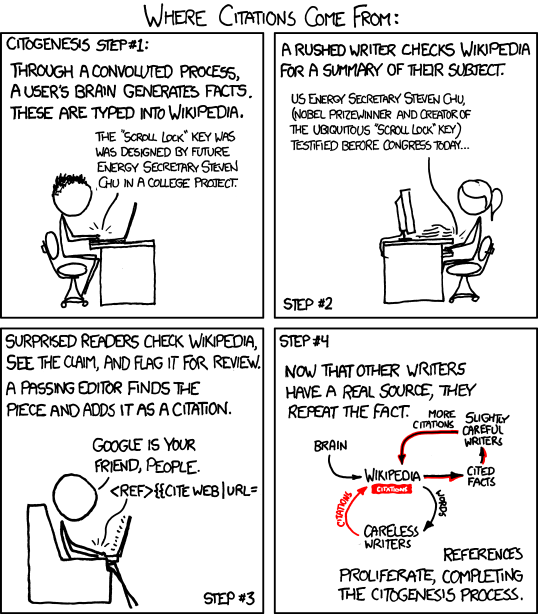
\includegraphics[width=7cm]{citogenesis}
   \caption[Zitierproblematik]{Ein Glaubwürdigkeitsproblem mancher Artikel in Wikipedia (Quelle: \url{https://xkcd.com/978/})    \label{fig:xkcd-citogenesis}}
  \end{subfigure}
\hfill
  \begin{subfigure}[t]{0.45\textwidth}
   \centering
   \caption{Logo der Fakultät für Bau- und Umweltingenieurwesen der TU Wien \label{fig:logo-fakultät}}
  \end{subfigure}
\caption{Beispiel einer \texttt{subfigure}-Umgebung \label{fig:bsp-subfigure}}
\end{figure}
%


\minisec{Matrix-Schreibweise}
%
Die Steifigkeitsmatrix sowie die Nachgiebigkeitsmatrix des Materials sind mit Bezug auf die Materialhauptrichtungen $L$-$R$-$T$ gegeben (siehe~\eqref{Glg:sigma} bis \eqref{Glg:D-matrix}).

Gesucht ist der Verzerrungstensor $\varepsilon$ im globalen Koordinatensystem $X,Y,Z$ sowie die Koordinaten der Eckpunkte in der verformten Lage (angegeben in [\si{mm}] auf 3~Dezimalstellen) unter der Annahme einer linearisierten Elastizitätstheorie.

\begin{equation}
\boldsymbol{\sigma}
=
\left(
   \begin{array}{c}
      \sigma_{xx} \\
      \sigma_{yy} \\
      \sigma_{zz} \\
      \sigma_{xy} \\
      \sigma_{yz} \\
      \sigma_{zx} \\
   \end{array}
\right)
=
\left(
   \begin{array}{c}
      1x{,}y \\
      1{,}xy \\
      2{,}xy \\
      3{,}xy \\
      0      \\
      0      \\
   \end{array}
\right)
\si{N/mm^2}
\label{Glg:sigma}
\end{equation}

\begin{equation}
\textbf{C}_{(LRT)}
=
\left(
\begin{array}{rrrccc}
\num{15500} & 489 & 274 & 0   & 0  & 0  \\
      & 844 & 162 & 0   & 0  & 0  \\
      &     & 632 & 0   & 0  & 0  \\
      &     &     & 700 & 0  & 0  \\
      &     &     &     & 60 & 0  \\
   \multicolumn{2}{l}{\text{symm.}}  
            &     &     &    & 650 \\
\end{array}
\right)
%
\cdot
%
\left(
   \begin{array}{c}
      \epsilon_{xx} \\
      \epsilon_{yy} \\
      \epsilon_{zz} \\
      \epsilon_{xy} \\
      \epsilon_{yz} \\
      \epsilon_{zx} \\
   \end{array}
\right)
=
\left(
   \begin{array}{r}
      \num{12,70} \\
      \num{1,27}  \\
      \num{2,27}  \\
      \num{3,27}  \\
      \multicolumn{1}{c}{0}     \\
      \multicolumn{1}{c}{0}     \\
   \end{array}
\right)
\label{Glg:C-matrix}
\end{equation}

\begin{equation}
\textbf{D}_{(LRT)}
=
\left(
   \begin{array}{rrrccc}
\num{6,595} &  \num{-3,441} &  \num{-1,977} &  0  &  0  & 0 \\
            & \num{126,411} & \num{-30,911} &  0  &  0  & 0 \\
            &               & \num{167,008} &  0  &  0  & 0 \\
            &               &               & \num{142,857} &  0  &  0  \\
            &               &               &    & \num{1666,667}  &  0  \\
   \multicolumn{2}{l}{\text{symm.}} &       &    &      & \num{153,846}  \\
\end{array}
\right)
\cdot \SI{e-5}{mm^2/N}
\label{Glg:D-matrix}
\end{equation}



\minisec{Beispiel für xfrac-Paket}
%
Dieses Paket verwendet den Befehl \textbackslash{}sfrac\{\}\{\} im Text
\sfrac{3}{4} oder in einer Formel $\sfrac{3}{4}$.

\minisec{Beispiele für den Einsatz des siunitx-packages}
Eine Verwendungsmöglichkeit ist die richtige Anzeige von Zahlen:
%
\begin{itemize} 
  \item als Einzelzahl: \num{12345678,9202}
  \item als Bereich von Zahlen: \numrange{12,3}{14,7} 
  \item als Liste von Zahlen: 
                      \numlist[list-final-separator={ und }]{12,3;13,5;14,7}
\end{itemize}
%
oder die richtige Darstellung von Einheiten (unabhängig ob im Paragraph- oder Math-Modus):
%
\begin{itemize} 
  \item Paragraphmodus: \si{\kilo\newton\per\meter}, \si{kN/m^2}
  \item Mathematikmodus:  $\si{\kilo\newton\per\meter}$, $\si{kN/m^2}$
\end{itemize}
%
oder die richtige Darstellung von Zahlen mit Einheiten:
%
\begin{itemize} 
  \item als Einzelzahl: \SI{12345678,92}{kNm}
  \item als Winkel: \ang{10}, \ang{12.3} oder \ang{12;3;5}
  \item als Bereich von Zahlen: \SIrange{12,3}{14,7}{\%} oder 
          \SIrange[range-units = single]{12,3}{14,7}{\%}
  \item als Liste von Zahlen: 
        \SIlist[list-final-separator={ und }]{12,3;13,5;14,7}{\kilogram/m^2}
\end{itemize}
%

\minisec{Beipiele für Abkürzungen samt zugehörigem Verzeichnis}

Das Programm \ac{rlt} wurde in Zusammenarbeit mit der \ac{obv} erstellt, berücksichtigt die deutsche \ac{abbv} -- von mehreren \aclp{abbv} -- und berechnet \ac{lzk}.

Nochmals:
Das Programm LZKB wurde in Zusammenarbeit mit der \ac{obv} erstellt, berücksichtigt die deutsche \ac{abbv} -- von mehreren \acp{abbv} -- und berechnet \ac{lzk}.

\printacronyms[name=Abkürzungen]



\minisec{Beispiel für den Einsatz des tabularx-packages}
Dieses Paket bietet die Möglichkeit der automatischen Anpassung der Spaltenbreite auf eine Gesamtbreite der Tabelle (siehe Tab.~\ref{tab:test}).


\begin{table}[h]
\caption{Ergebnisse der schriftlichen Prüfung \label{tab:test}}
   \begin{tabularx}{\textwidth}{@{}lccX@{}}
   \toprule
   Name & Entwurf     & Pläne       & Anmerkung    \\
   \midrule
   Mayer    & \SI{60}{\%} & \SI{60}{\%} & 
      Funktionalle Umsetzung mit hinreichender Routine. Konstruktive Darstellung speziell im Dachbereich nicht nachvollziehbar. \\
   Müller   & \SI{20}{\%} & \SI{30}{\%} & 
      In allen Teilbereichen sehr detailierte Konzeption, allerdings fehlt die planliche Umsetzung, sodass aufgrund des fehlenden Informationsgehalts keine positive Beurteilung möglich ist. \\
   Schmidt  & \SI{90}{\%} & \SI{90}{\%} & 
      In allen Prüfungsabschnitte routinierte Darstellung und planliche Umsetzung. Die Nachvollziehbarkeit ist in allen Teilabschnitten gegeben. \\
   \bottomrule
   \end{tabularx}
\end{table}




\minisec{Beispiel für den Einsatz der longtable- und multirow-packages}

\begin{longtable}{@{}l*{3}{S[table-format=2.2]}@{}}
\caption{Messwerte der bauphysikalischen Untersuchung \label{tab:bauphysik}}
\\ \toprule
Datum & {Mittel [\si{\degreeCelsius}]} & {Min [\si{\degreeCelsius}]} & {Max [\si{\degreeCelsius}]}
\\ \midrule
\endfirsthead
\caption{Messwerte der bauphysikalischen Untersuchung (Fortsetzung)}
\\ \toprule
Datum & {Mittel [\si{\degreeCelsius}]} & {Min [\si{\degreeCelsius}]} & {Max [\si{\degreeCelsius}]}
\\ \midrule
\endhead
%
  \midrule
  \multicolumn{4}{r}{{Continued on next page}} 
  \\ \bottomrule
\endfoot
%
  \bottomrule
\endlastfoot
06-Jul-2016 & 24,6 & 20,9 & 25,0 \\
07-Jul-2016 & 24,82 & 24,50 & 25,30 \\
08-Jul-2016 & 24,58 & 24,30 & 25,10 \\
09-Jul-2016 & 24,58 & 24,40 & 24,80 \\
10-Jul-2016 & 24,53 & 24,40 & 24,90 \\
11-Jul-2016 & 24,55 & 24,20 & 25,00 \\
12-Jul-2016 & 24,55 & 24,40 & 24,70 \\
13-Jul-2016 & 24,55 & 24,40 & 24,70 \\
14-Jul-2016 & 25,02 & 24,50 & 25,40 \\
15-Jul-2016 & 25,22 & 24,80 & 25,50 \\
16-Jul-2016 & 25,45 & 25,30 & 25,70 \\
17-Jul-2016 & 25,35 & 24,80 & 25,70 \\
18-Jul-2016 & 25,29 & 24,80 & 25,70 \\
19-Jul-2016 & 24,83 & 24,60 & 25,10 \\
20-Jul-2016 & 24,73 & 24,60 & 25,00 \\
21-Jul-2016 & 24,68 & 24,50 & 24,90 \\
22-Jul-2016 & 24,70 & 24,60 & 25,00 \\
23-Jul-2016 & 24,72 & 24,60 & 25,00 \\
24-Jul-2016 & 24,81 & 24,60 & 25,00 \\
25-Jul-2016 & 24,74 & 24,50 & 25,00 \\
26-Jul-2016 & 24,70 & 24,60 & 24,80 \\
27-Jul-2016 & 24,72 & 24,50 & 25,00 \\
28-Jul-2016 & 24,66 & 24,50 & 24,90 \\
29-Jul-2016 & 24,66 & 24,50 & 24,80 \\
30-Jul-2016 & 24,69 & 24,60 & 24,80 \\
31-Jul-2016 & 24,77 & 24,70 & 25,00 \\
01-Aug-2016 & 24,72 & 24,40 & 25,00 \\
02-Aug-2016 & 24,64 & 24,50 & 24,90 \\
03-Aug-2016 & 24,73 & 24,60 & 25,00 \\
04-Aug-2016 & 24,74 & 24,60 & 24,80 \\
05-Aug-2016 & 24,76 & 24,60 & 25,20 \\
06-Aug-2016 & 25,30 & 24,80 & 25,70 \\
07-Aug-2016 & 25,10 & 24,70 & 25,60 \\
08-Aug-2016 & 25,06 & 24,80 & 25,50 \\
09-Aug-2016 & 24,89 & 24,70 & 25,20 \\
10-Aug-2016 & 25,52 & 25,00 & 25,80 \\
11-Aug-2016 & 25,60 & 25,30 & 25,80 \\
12-Aug-2016 & 25,81 & 25,60 & 26,00 \\
13-Aug-2016 & 25,95 & 25,50 & 26,30 \\
14-Aug-2016 & 25,79 & 25,40 & 26,30 \\
15-Aug-2016 & 25,47 & 25,20 & 25,90 \\
16-Aug-2016 & 25,36 & 25,10 & 25,90 \\
17-Aug-2016 & 25,33 & 25,10 & 25,80 \\
18-Aug-2016 & 25,42 & 25,00 & 25,90 \\
19-Aug-2016 & 25,36 & 25,00 & 25,70 \\
20-Aug-2016 & 25,37 & 25,00 & 25,80 \\
21-Aug-2016 & 25,38 & 25,10 & 25,70 \\
22-Aug-2016 & 25,88 & 25,60 & 26,20 \\
23-Aug-2016 & 25,85 & 25,10 & 26,70 \\
24-Aug-2016 & 25,10 & 24,80 & 26,30 \\
25-Aug-2016 & 25,22 & 24,80 & 25,70 \\
26-Aug-2016 & 24,91 & 24,70 & 25,30 \\
27-Aug-2016 & 24,75 & 24,60 & 25,00 \\
28-Aug-2016 & 24,74 & 24,60 & 25,00 \\
29-Aug-2016 & 24,76 & 24,50 & 25,00 \\
30-Aug-2016 & 24,77 & 24,60 & 25,10 \\
31-Aug-2016 & 24,87 & 24,60 & 25,30 \\
01-Sep-2016 & 24,97 & 24,60 & 25,60 \\
02-Sep-2016 & 24,78 & 24,60 & 25,10 \\
03-Sep-2016 & 24,95 & 24,70 & 25,40 \\
04-Sep-2016 & 24,91 & 24,70 & 25,20 \\
05-Sep-2016 & 25,21 & 24,80 & 25,70 \\
06-Sep-2016 & 25,81 & 25,40 & 26,40 \\
07-Sep-2016 & 26,01 & 25,50 & 26,50 \\
08-Sep-2016 & 25,66 & 25,30 & 26,30 \\
09-Sep-2016 & 25,29 & 25,10 & 25,40 \\
10-Sep-2016 & 25,20 & 25,10 & 25,30 \\
11-Sep-2016 & 25,19 & 25,00 & 25,40 \\
12-Sep-2016 & 25,08 & 24,80 & 25,40 \\
13-Sep-2016 & 24,92 & 24,80 & 25,00 \\
14-Sep-2016 & 24,81 & 24,60 & 24,90 \\
15-Sep-2016 & 24,76 & 24,50 & 25,00 \\
16-Sep-2016 & 24,94 & 24,80 & 25,20 \\
17-Sep-2016 & 25,04 & 24,80 & 25,50 \\
18-Sep-2016 & 25,44 & 25,10 & 25,80 \\
19-Sep-2016 & 25,70 & 25,40 & 26,00 \\
20-Sep-2016 & 25,85 & 25,70 & 26,10 \\
21-Sep-2016 & 25,92 & 25,70 & 26,20 \\
22-Sep-2016 & 25,94 & 25,70 & 26,20 \\
23-Sep-2016 & 25,87 & 25,50 & 26,30 \\
24-Sep-2016 & 26,01 & 25,60 & 26,40 \\
\multirow{3}{*}{25--27-Sep-2016} 
            & 26,00 & 25,60 & 26,30 \\
            & 26,19 & 25,70 & 26,50 \\
            & 26,19 & 25,50 & 26,50 \\
\end{longtable}

\minisec{Beispiel für den Einsatz des threeparttable-packages}

\begin{table}[htpb]
  \centering
  \caption{Beispiel für einen threeparttable}
  \label{tab:near_optimal}
  \begin{threeparttable}
    \begin{tabular}{@{}l|lllll@{}}\toprule
      Location\tnote{1}             & Beam 1    & Beam 2    & Beam 3    & Beam 4    & Beam 5    \\ \midrule
      1                             & 16$^\ast$ & 21        & 28        & 32        & 36$^\ast$ \\
      2                             & 14$^\ast$ & 33        & 47        & 37$^\ast$ & 35$^\ast$ \\ \midrule
      Deflection [$10^{-5}\si{mm}$] & $4.4753$  & $4.4575$  & $4.5067$  & $4.5076$  & $4.4642$  \\
    \bottomrule\end{tabular}
    \begin{tablenotes}
    \item[] Lamella IDs marked with an asterisk are flipped
    \item[1] The location is defined from top to bottom of the beam.
    \end{tablenotes}
  \end{threeparttable}
\end{table}







\chapter{Einleitung}
%Kapitel von Mangeng
\chapter{Projektmanagement}

\section{blabliblub}





\chapter{Planung}

Hi

\section{Lüftungsgeräte}


\section{Modbus}
Die offizielle Definition des Modbus Protokolls bezogen von der Modbus Organization \cite{Modbus_Organization_AP:2012} lautet:
\begin{quotation}
	\emph{
		MODBUS is an application layer messaging protocol, positioned at level 7 of the OSI model, which provides client/server communication between devices connected on different types of buses or networks.}
\end{quotation}

Der Modbus Standard definiert ein Application Layer Kommunikations Protokoll, dass sich auf Schicht 7 des OSI-Modells befindet. Es bietet Client/Server Kommunikation zwischen Geräten, die auf verschiedenen Bussen oder Netzwerken angeschlossen sind.

Das Modbus-Protokoll wurde 1979 von Gould-Modicon entwickelt. Aufgrund seiner offenen Art (man kann jegliche Geräte als Client anhängen) und geringer Kosten, ist das Modbus-Protokoll immer noch ein Industriestandard. Besonders oft wird das Protokoll in Mess- und Regelsystemen eingesetzt (https://www.kvm-concepts.de/wiki/m/modbus/)
https://www.kunbus.com/de/modbus 

Es gibt zwei verschiedene Einteilungen des Modbus Protokolls: 
\begin{itemize}
\item \textbf{Modbus Application Protocol:} Befindet sich auf der siebten Schicht des OSI-Modells. Dabei können die Geräte an einem Bus oder an einem Netzwerk angeschlossen werden. Genauere Information über die Ausführungsart mit dem TCP Protokoll sind später in diesem Kapitel zu finden.
\item \textbf{Modbus Serial Line Protocol:} Befindet sich auf der zweiten Schicht des OSI-Modells. Die Geräte sind hier an einem seriellen Bus angeschlossen. Dabei gibt es hier zwei Ausführungsarten, nämlich RTU und ASCII. Diese werden später ausführlicher beschrieben.
\end{itemize}
\cite{Modbus_Organization_AP:2012}
\cite{Modbus_Organization_SL:2012}

\subsection{Funktionsweise}
Modbus verwendet das Client/Server System. In einem Bussystem kann es nur einen Client geben. Es können jedoch beliebig viele Server am Bus angeschlossen werden. Der Client kann die Kommunikation mit den einzelnen Servern initialisieren. Er kann ihnen Daten senden und von ihnen Daten anfordern. Ein Server hingegen kann keine Kommunikation beginnen, sondern lediglich auf Anfrage des Clients handeln.

Modbus basiert auf Registern 

Der Grundbestandteil des Modbus Protokolls sind ist die sogenannte \acf{pdu}. Diese besteht aus einem Function Code und den Daten. In manchen Fällen werden dem \acs{pdu} zusätzliche Felder hinzugefügt. Es kann zum Beispiel eine zusätzliche Adresse und eine Checksumme zur Fehlererkennung eingebaut werden. Das erweiterte Datenpaket wird \acf{apu} genannt.
(BILD VON MODBUS SEITE EINBAUEN ZU ADU UND PDU)
\begin{itemize}
	\item \textbf{Additional Address:}
	\item \textbf{Function Code:} Dieses Feld ist ein Byte groß. Die Werte reichen von 1 bis 255, wobei 128 bis 255 für Fehlercodes vorbehalten sind. Wenn der Server eine Nachricht vom Client bekommt, zeigt ihm dieses Feld an, was er mit den erhaltenen Daten machen soll. 
	\item \textbf{Data:} In diesem Feld werden die Daten beigefügt. Außerdem sind  auch zusätzliche Informationen wie die Registeradressen und die Länge der Daten enthalten.
	\item \textbf{Error Check:}
\end{itemize}


\cite{Modbus_Organization_AP:2012}

\subsection{Vor- und Nachteile}


\subsection{Ausführungsarten}
\paragraph{RTU}
Funktioniert über die serielle Schnittstelle.
\paragraph{ASCII}
\paragraph{TCP}

\subsection{Serielle Kommunikation (bei RTU/RS485)}




\section{Hardware-Evaluation und -Selektion}

\section{Software-Selektion}


\chapter{Umsetzung}

\section{Hardware Setup}
\subsection{Prototypenaufbau}
\subsection{Übertragen der Config-Files mittels USB}


\section{Auslesen der Werte über USB}

\section{Auslesen der Werte über RS485}

\section{JSON Config-Files}

\section{Python Functions}

\section{Einbinden der JSON Config-Files}

\section{Einbinden der Python Functions}


\appendix
%% insert bibliography, adds chapter heading with chapter number
\printbibliography

\minisec{Zitierbeispiele entsprechend DIN ISO 690}

Die DIN~ISO~690~\cite{DIN-ISO-690:2013} gibt Hinweise zur vollständigen Quellenangabe.
Das folgende Beispiele ist dieser Norm entlehnt und angepasst:
%
\begin{quotation}
Einige Standardwerke \cite{Kohm:20,Voss:22} geben einen guten Überblick über \LaTeX{}.
\textcite{Kohm:20} hat die Klassen der KOMA-Script-Reihe entwickelt, die die \enquote{typografischen Gepflogenheiten eines europäischen Layouts berücksichtigen}~\cite[S.~64]{Voss:22}.
Daneben empfehlen wir -- nona -- unser Buch zu \LaTeX{}, Excel und Word: \textcite{Schranz:22}.
\end{quotation}

Nun der selbe Text in Harvard Citation Style (jedoch ohne \LaTeX-Befehle -- diese wären die selben wie zuvor, es müsste nur der Zitierstil geändert werden):
%
\begin{quotation}
Einige Standardwerke (Kohm 2020, Voss 2022) geben einen guten Überblick über \LaTeX{}.
Kohm (2020) hat die Klassen der KOMA-Script-Reihe entwickelt, die die \enquote{typografischen Gepflogenheiten eines europäischen Layouts berücksichtigen}~(Voss 2022, S.~64).
Daneben empfehlen wir -- nona -- unser Buch zu \LaTeX{}, Excel und Word: Schranz et al. (2022).
\end{quotation}

\listoffigures
\listoftables

\end{document}
